% Options for packages loaded elsewhere
\PassOptionsToPackage{unicode}{hyperref}
\PassOptionsToPackage{hyphens}{url}
%
\documentclass[
]{article}
\usepackage{lmodern}
\usepackage{amssymb,amsmath}
\usepackage{ifxetex,ifluatex}
\ifnum 0\ifxetex 1\fi\ifluatex 1\fi=0 % if pdftex
  \usepackage[T1]{fontenc}
  \usepackage[utf8]{inputenc}
  \usepackage{textcomp} % provide euro and other symbols
\else % if luatex or xetex
  \usepackage{unicode-math}
  \defaultfontfeatures{Scale=MatchLowercase}
  \defaultfontfeatures[\rmfamily]{Ligatures=TeX,Scale=1}
\fi
% Use upquote if available, for straight quotes in verbatim environments
\IfFileExists{upquote.sty}{\usepackage{upquote}}{}
\IfFileExists{microtype.sty}{% use microtype if available
  \usepackage[]{microtype}
  \UseMicrotypeSet[protrusion]{basicmath} % disable protrusion for tt fonts
}{}
\makeatletter
\@ifundefined{KOMAClassName}{% if non-KOMA class
  \IfFileExists{parskip.sty}{%
    \usepackage{parskip}
  }{% else
    \setlength{\parindent}{0pt}
    \setlength{\parskip}{6pt plus 2pt minus 1pt}}
}{% if KOMA class
  \KOMAoptions{parskip=half}}
\makeatother
\usepackage{xcolor}
\IfFileExists{xurl.sty}{\usepackage{xurl}}{} % add URL line breaks if available
\IfFileExists{bookmark.sty}{\usepackage{bookmark}}{\usepackage{hyperref}}
\hypersetup{
  hidelinks,
  pdfcreator={LaTeX via pandoc}}
\urlstyle{same} % disable monospaced font for URLs
\usepackage{graphicx}
\makeatletter
\def\maxwidth{\ifdim\Gin@nat@width>\linewidth\linewidth\else\Gin@nat@width\fi}
\def\maxheight{\ifdim\Gin@nat@height>\textheight\textheight\else\Gin@nat@height\fi}
\makeatother
% Scale images if necessary, so that they will not overflow the page
% margins by default, and it is still possible to overwrite the defaults
% using explicit options in \includegraphics[width, height, ...]{}
\setkeys{Gin}{width=\maxwidth,height=\maxheight,keepaspectratio}
% Set default figure placement to htbp
\makeatletter
\def\fps@figure{htbp}
\makeatother
\setlength{\emergencystretch}{3em} % prevent overfull lines
\providecommand{\tightlist}{%
  \setlength{\itemsep}{0pt}\setlength{\parskip}{0pt}}
\setcounter{secnumdepth}{-\maxdimen} % remove section numbering

\author{}
\date{}

\begin{document}

\hypertarget{ux57faux4e8ebertux7684ux6587ux672cux5206ux7c7bux6a21ux578b}{%
\section{基于Bert的文本分类模型}\label{ux57faux4e8ebertux7684ux6587ux672cux5206ux7c7bux6a21ux578b}}

\hypertarget{ux6570ux636eux96c6}{%
\subsection{数据集}\label{ux6570ux636eux96c6}}

中文数据集:

\begin{enumerate}
\def\labelenumi{\arabic{enumi}.}
\item
  \href{https://github.com/SophonPlus/ChineseNlpCorpus/blob/master/datasets/yf_amazon/intro.ipynb}{yf\_amazon},数据来源亚马逊,52
  万件商品,1100 多个类目,142 万用户,720 万条评论/评分数据.
\item
  \href{https://github.com/SophonPlus/ChineseNlpCorpus/blob/master/datasets/weibo_senti_100k/intro.ipynb}{weibo\_senti\_100k
  },数据来源新浪微博,10 万多条,带情感标注 新浪微博,正负向评论约各 5
  万条.
\item
  \href{https://github.com/SophonPlus/ChineseNlpCorpus/blob/master/datasets/simplifyweibo_4_moods/intro.ipynb}{simplifyweibo\_4\_moods
  },数据来源新浪微博,36 万多条,带情感标注 新浪微博,包含 4
  种情感,其中喜悦约 20 万条,愤怒、厌恶、低落各约 5
  万条(但标签给的不是很准确)
\item
  \href{https://github.com/SophonPlus/ChineseNlpCorpus/blob/master/datasets/waimai_10k/intro.ipynb}{waimai\_10k
  },某外卖平台收集的用户评价,正向 4000 条,负向 约 8000 条.
\item
  \href{https://github.com/SophonPlus/ChineseNlpCorpus/blob/master/datasets/online_shopping_10_cats/intro.ipynb}{online\_shopping\_10\_cats
  },10
  个类别(书籍、平板、手机、水果、洗发水、热水器、蒙牛、衣服、计算机、酒店),共
  6 万多条评论数据,正、负向评论各约 3 万条.
\end{enumerate}

最终选择第五个数据集\texttt{online\_shopping\_10\_cats},根据用户评论完成以下两个分类任务:

\begin{enumerate}
\def\labelenumi{\arabic{enumi}.}
\item
  商品类别(10类).
\item
  正面还是负面评价(2类).
\end{enumerate}

\begin{verbatim}
书籍: 3851 (总体), 2100 (正例), 1751 (负例)
平板: 10000 (总体), 5000 (正例), 5000 (负例)
手机: 2323 (总体), 1165 (正例), 1158 (负例)
水果: 10000 (总体), 5000 (正例), 5000 (负例)
洗发水: 10000 (总体), 5000 (正例), 5000 (负例)
热水器: 575 (总体), 475 (正例), 100 (负例)
蒙牛: 2033 (总体), 992 (正例), 1041 (负例)
衣服: 10000 (总体), 5000 (正例), 5000 (负例)
计算机: 3992 (总体), 1996 (正例), 1996 (负例)
酒店: 10000 (总体), 5000 (正例), 5000 (负例)
\end{verbatim}

\hypertarget{bertux6a21ux578b-1}{%
\subsection{Bert模型}\label{bertux6a21ux578b-1}}

Bert模型原理参考文章:

\begin{enumerate}
\def\labelenumi{\arabic{enumi}.}
\item
  \href{https://cloud.tencent.com/developer/article/1389555}{图解BERT模型:从零开始构建BERT}
  这篇文章详细的介绍了Bert的原理、transformer模型和Attention机制.
  (以下图片均来自该博客)
\item
  \href{https://zhuanlan.zhihu.com/p/98855346}{什么是BERT?}
  这两篇文章都介绍了Bert模型的输入输出还有Bert的结构,第二篇更简短一些.
  其预训练部分使用的原理,MLM和NSP过程,不用很具体的讲解,只需要大致介绍他们俩分别起到什么功能.
\end{enumerate}

Bert模型是一种\textbf{无监督学习的预训练模型}(能进行迁移学习的模型,用于各种NLP问题),模型主要就是将transformer模型进行堆叠而形成的,其输入与输出的维度相同,过程类似于词编码过程,将低维的词向量进行编码,并将其特征进行放大,与其他特征进行分离.(\href{https://zhuanlan.zhihu.com/p/164502624}{知乎
- Embedding过程})

\hypertarget{ux6a21ux578bux7ed3ux6784}{%
\subsubsection{模型结构}\label{ux6a21ux578bux7ed3ux6784}}

NLP,BERT,Transformer,Attention之间的关系

\begin{figure}
\centering
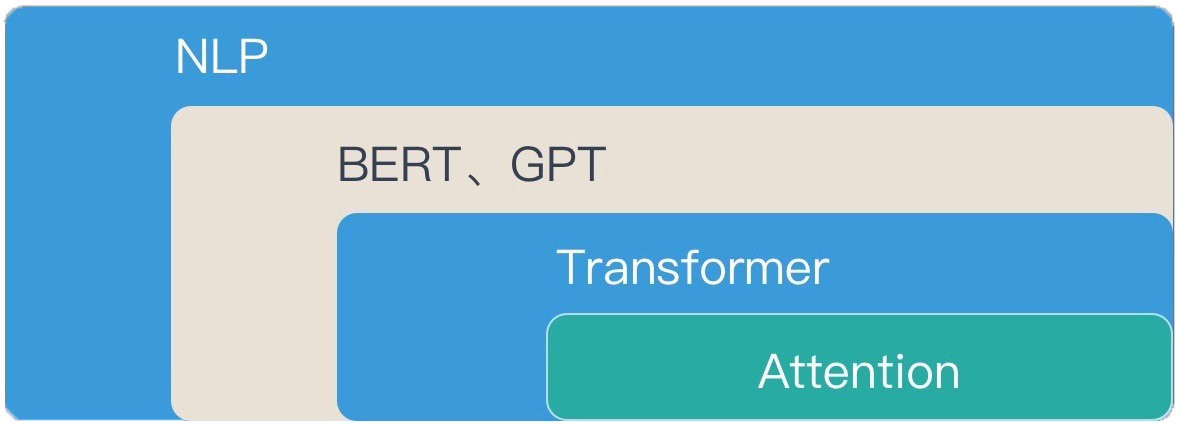
\includegraphics{D:/yy/Documents/GitHub/LaTex-Projects/NLP/NLP大作业/NLP大作业note.figure/Bert,Transformer,Attention之间的关系.jpg}
\caption{}
\end{figure}

\hypertarget{attentionux673aux5236}{%
\paragraph{Attention机制}\label{attentionux673aux5236}}

Attention机制主要思路就是:\textbf{通过机器学习得到单词之间的权重分布,然后作用在特征上}.

Attention机制有三种实现方式:RNN+Attention,CNN+Attention,纯Attention,第三种就是Google团队在2017发表的论文\href{https://arxiv.org/pdf/1706.03762.pdf}{Attention
is All you need}中提到的,上述模型都是使用该思路搭建的.

这里以单个文字的Attention权重计算为例,首先将该句话总每个文字使用神经网络转化为向量表示形式(词向量),取定一个文字作为当前的Query目标,将上下文的文字作为Key,并同时另存到Value值内.
然后计算Query值和Key值的相关性(利用内积进行计算),并通过softmax函数得到Attention权重(归一化),最后再对Value向量使用Attention权重加权求和,即可得到Attention机制后的输出.

\begin{figure}
\centering
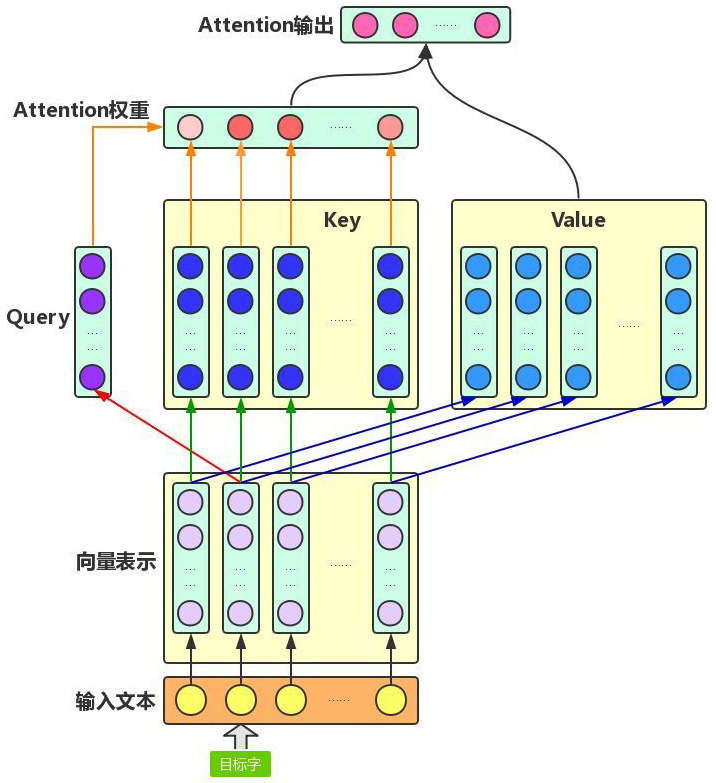
\includegraphics{D:/yy/Documents/GitHub/LaTex-Projects/NLP/NLP大作业/NLP大作业note.figure/Attention机制.jpg}
\caption{}
\end{figure}

我们再对该句话中每一个文字都进行如上操作即可得到整句话的Attention输出,由于只融合了该句话字之间的相关性,所以也称为Self-Attention,如下图所示:

\begin{figure}
\centering
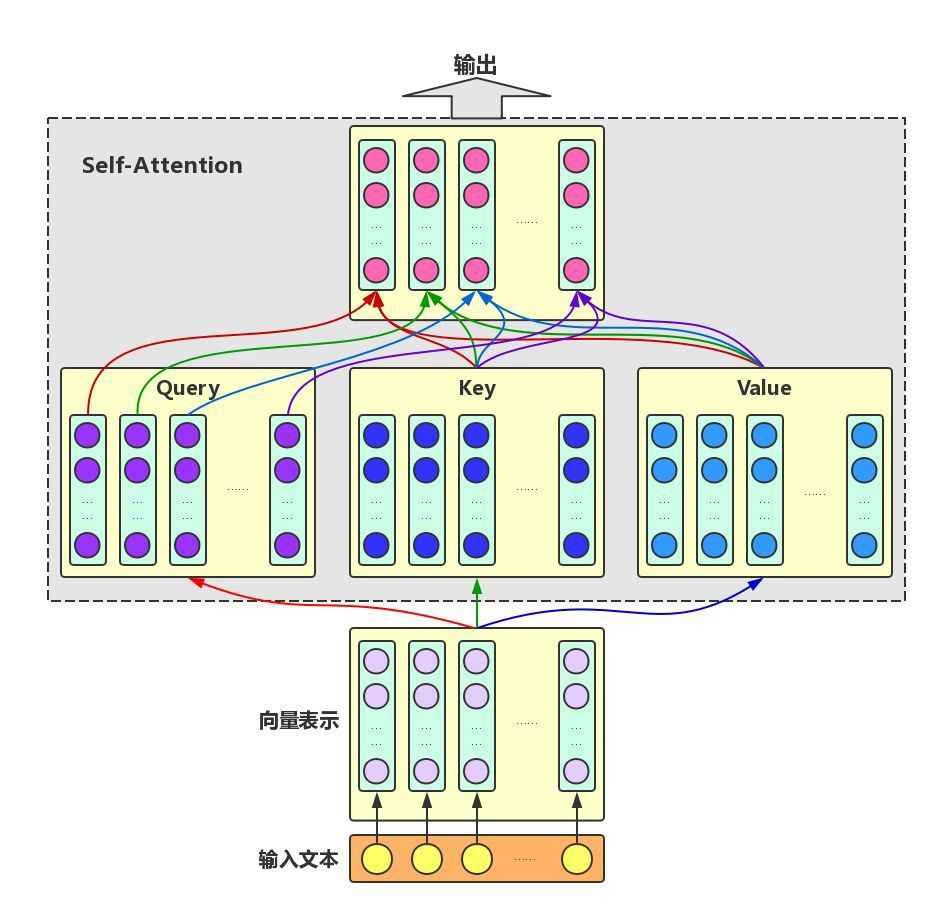
\includegraphics{D:/yy/Documents/GitHub/LaTex-Projects/NLP/NLP大作业/NLP大作业note.figure/Self-Attention.jpg}
\caption{}
\end{figure}

为了进一步(增加模型的复杂性dog)提高Attention处理的多样性,处理不同语义空间下的增强向量,Transformer模型中进一步叠加Self-Attention,最后连接神经网络保持输出层和原始向量长度相同,这就得到了Multi-head
Self-Attention

\begin{figure}
\centering
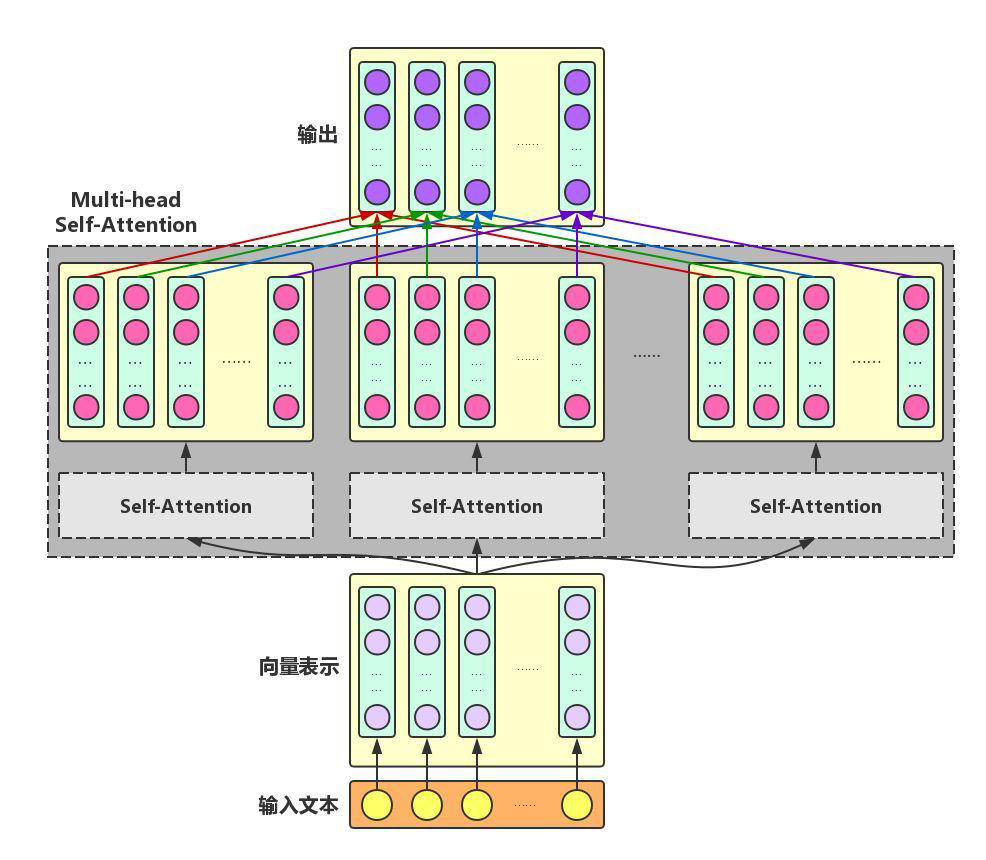
\includegraphics{D:/yy/Documents/GitHub/LaTex-Projects/NLP/NLP大作业/NLP大作业note.figure/Multi-head Self-Attention.jpg}
\caption{}
\end{figure}

\hypertarget{transformer-encoder}{%
\paragraph{Transformer Encoder}\label{transformer-encoder}}

由于Berd中只是用了Transformer的编码部分,所以只对其进行介绍.
Transformer主要是在Multi-head Self-Attention的基础上加入了三个操作:

\begin{enumerate}
\def\labelenumi{\arabic{enumi}.}
\item
  残差连接(Residual
  Connection):此处使用的思路应该是来自2015年ImageNet图像识别比赛第一名的\href{https://arxiv.org/abs/1512.03385}{ResNet},其主要用于解决深度神经网络在深度过高之后数据过度离散的问题,主要解决了过多的非线性函数导致网络难以实现恒等变换的问题,同样该操作使得网络变得更加容易训练.
\item
  层标准化(Layer
  Normalization):对某一层神经网络做均值为0方差为1的标准化操作,主要为了避免网络过深导致loss值过小的问题.
\item
  两次线性变换:两层神经网络处理,增强模型的表达能力(保持输入与输出长度相同).
\end{enumerate}

\begin{figure}
\centering
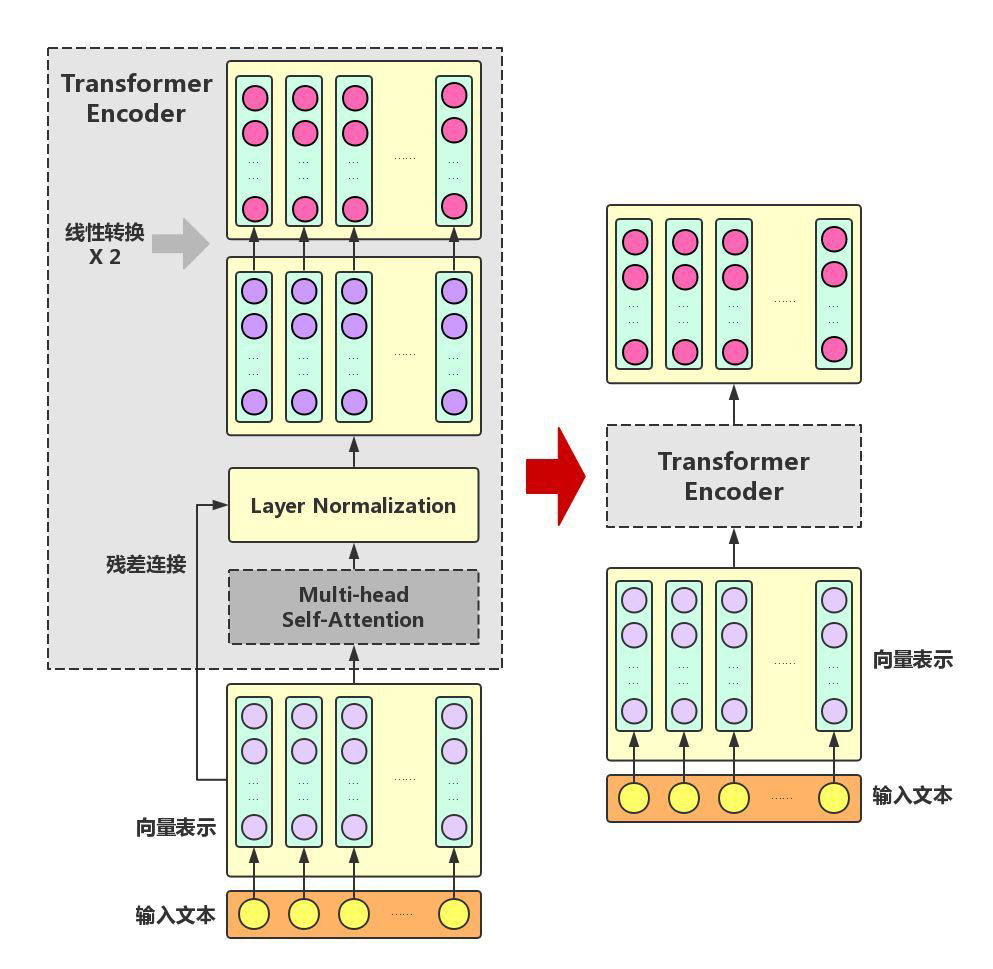
\includegraphics{D:/yy/Documents/GitHub/LaTex-Projects/NLP/NLP大作业/NLP大作业note.figure/Transformer.jpg}
\caption{}
\end{figure}

\hypertarget{bertux6a21ux578b-2}{%
\paragraph{Bert模型}\label{bertux6a21ux578b-2}}

再在Transformer模型基础上对其进行堆叠,就完成了Bert模型基本框架.(堆叠层数为12层和24层,我们将使用12层的Bert模型进行训练)

\begin{figure}
\centering
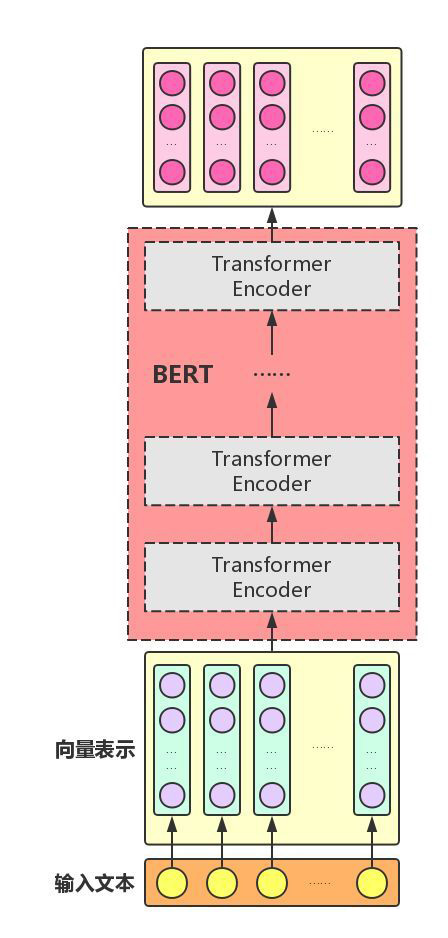
\includegraphics{D:/yy/Documents/GitHub/LaTex-Projects/NLP/NLP大作业/NLP大作业note.figure/Bert.jpg}
\caption{}
\end{figure}

\hypertarget{ux9884ux8badux7ec3ux4efbux52a1}{%
\subsubsection{预训练任务}\label{ux9884ux8badux7ec3ux4efbux52a1}}

有了Bert模型之后,为了使该模型具有泛化能力,能够用于处理各种NLP问题,论文作者以Wiki作为数据集对模型进行预训练(如同在读懂文章之前,学会如何理解句式,学习语言的本身).
Bert模型主要由以下两个预训练模型构成:

\begin{enumerate}
\def\labelenumi{\arabic{enumi}.}
\item
  Masked Language
  Model(MLM),在一句话中随机掩去该句话中的几个字,通过剩余的字去预测掩去的字是什么,类似英文中的完形填空,本质是在模仿人类学习语言的方法,这样的好处在于迫使机器去依赖上下文预测词汇,增强上下文词汇之间的关联性,并赋予其一定的纠错能力.
\end{enumerate}

\begin{figure}
\centering
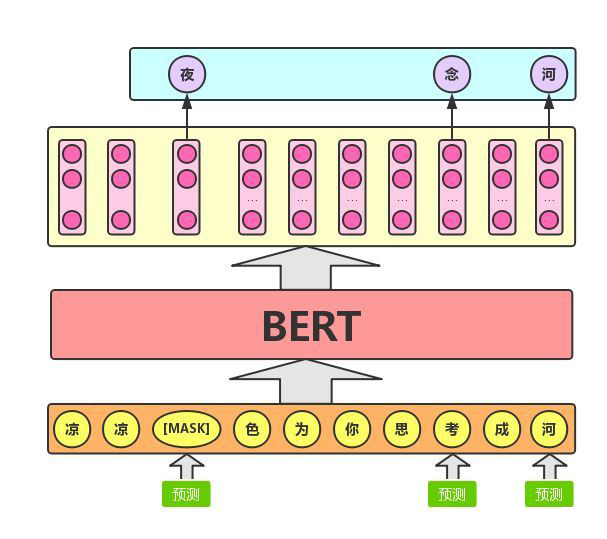
\includegraphics{D:/yy/Documents/GitHub/LaTex-Projects/NLP/NLP大作业/NLP大作业note.figure/Masked Language Model.jpg}
\caption{}
\end{figure}

\begin{enumerate}
\def\labelenumi{\arabic{enumi}.}
\item
  Next Sentence
  Prediction(NSP):通过给出文章中的两句话,判断第一句话是否出现在第二句话之后,类似高中语文的古诗词默写和英文的段落重排,该训练可以使模型学习到整篇文章内容之间的关联性,更准确的刻画语句之间的信息.
\end{enumerate}

\begin{figure}
\centering
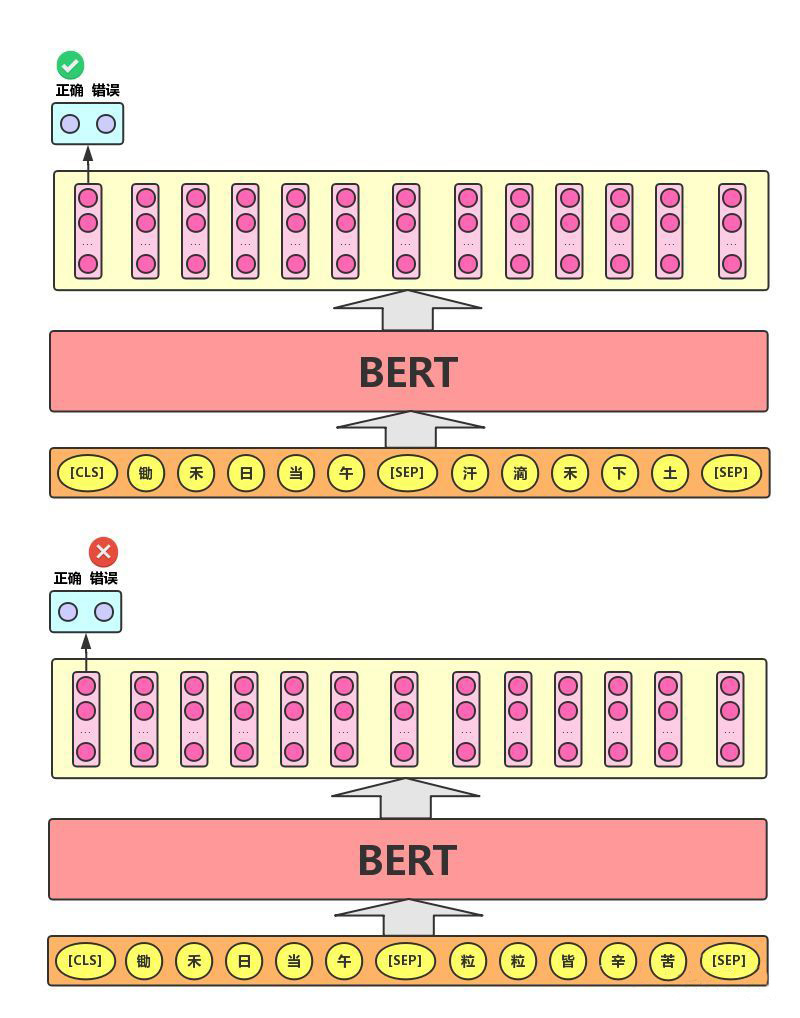
\includegraphics{D:/yy/Documents/GitHub/LaTex-Projects/NLP/NLP大作业/NLP大作业note.figure/Next Sentence Prediction.jpg}
\caption{}
\end{figure}

\hypertarget{ux6a21ux578bux5e94ux7528}{%
\subsubsection{模型应用}\label{ux6a21ux578bux5e94ux7528}}

对于不同的现实场景Bert模型通过构建不同的输出层维度从而完成不同的分类问题,例如:单文本分类(通过在文章的开头加入{[}CLS{]}符号表示文章的语义信息),语义场景分类(使用{[}SEP{]}分隔符作为两句话之间的分隔),序列标注问题等等.
通过对Bert模型的输出进行微调从而完成各种分类问题(在输出层后加入神经网络训练).

\hypertarget{ux4e3bux8981ux5de5ux4f5c}{%
\subsection{主要工作}\label{ux4e3bux8981ux5de5ux4f5c}}

\begin{enumerate}
\def\labelenumi{\arabic{enumi}.}
\item
  学习深度学习相关框架与技术.
\item
  电商数据\texttt{online\_shopping\_10\_cats}的预处理,均衡每种商品类别信息的数目,均衡正负评论数目.
\item
  划分训练集与验证集,调整模型输出,超参数调整,提高准确率.
\item
  考虑使用其他电商数据作为测试集(例如\texttt{yf\_amazon}),测试模型的泛化性.
\end{enumerate}

TensorFlow中的中文处理的Bert模型:\href{https://tfhub.dev/tensorflow/bert_zh_preprocess/3}{bert\_zh\_preprocess(预处理)},\href{https://tfhub.dev/tensorflow/bert_zh_L-12_H-768_A-12/4}{bert\_zh\_L-12\_H-768\_A-12(12层的Bert模型)}.

\hypertarget{ux5b66ux4e60ux8d44ux6599}{%
\subsection{学习资料}\label{ux5b66ux4e60ux8d44ux6599}}

\hypertarget{youtube}{%
\paragraph{YouTube}\label{youtube}}

\begin{enumerate}
\def\labelenumi{\arabic{enumi}.}
\item
  \href{https://www.youtube.com/watch?v=hQwFeIupNP0\&list=RDCMUCh9nVJoWXmFb7sLApWGcLPQ\&start_radio=1\&rv=hQwFeIupNP0\&t=4}{What
  is Word2Vec? A Simple Explanation \textbar{} Deep Learning Tutorial 41
  (Tensorflow, Keras \& Python)}
\item
  \href{https://www.youtube.com/watch?v=Q2NtCcqmIww}{Word2Vec Part 2
  \textbar{} Implement word2vec in gensim \textbar{} \textbar{} Deep
  Learning Tutorial 42 with Python}
\item
  \href{https://www.youtube.com/watch?v=7kLi8u2dJz0\&t=799s}{What is
  BERT? \textbar{} Deep Learning Tutorial 46 (Tensorflow, Keras \&
  Python)}
\item
  \href{https://www.youtube.com/watch?v=hOCDJyZ6quA}{Text Classification
  Using BERT \& Tensorflow \textbar{} Deep Learning Tutorial 47
  (Tensorflow, Keras \& Python)}
\end{enumerate}

\end{document}
